\documentclass{beamer}
\usepackage[latin1]{inputenc}
\usetheme{Warsaw}
\title[Volunteer Cloud Computing]{Volunteer Cloud Computing}
\author{Dany Wilson -- Dr. St�phane Som�}
\institute{University of Ottawa}
\date{January 23, 2015}

\usepackage{tikz}
\usetikzlibrary{trees}

\begin{document}

\begin{frame}
\titlepage
\end{frame}

\begin{frame}
  \frametitle{Agenda}
  \tableofcontents [hideallsubsections]
\end{frame}

\section{Introduction}
\subsection{Volunteer Computing}
\begin{frame}
  \frametitle{Volunteer Computing}
  \begin{figure}[GIMPS]
    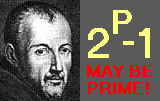
\includegraphics{GIMPS_logo.png}
  \end{figure}

  \begin{itemize}
  % Mersenne Prime numbers are prime numbers that are one less than a
  % power of 2  (3, 7, 31, 127)
  \item Great Internet Mersenne Prime Search [1996]
  \item Distributed Computing based on Collaboration
  \item ... throughput of 137.023 TeraFLOP/s
  \end{itemize}
\end{frame}

\subsection{Cloud Computing}

\begin{frame}
  \frametitle{Cloud Computing}
  \begin{itemize}
  \item Natural evolution of Web 2.0, SoA and Virtualization
    technologies. 
  \end{itemize}

  \begin{figure}[Cloud]
    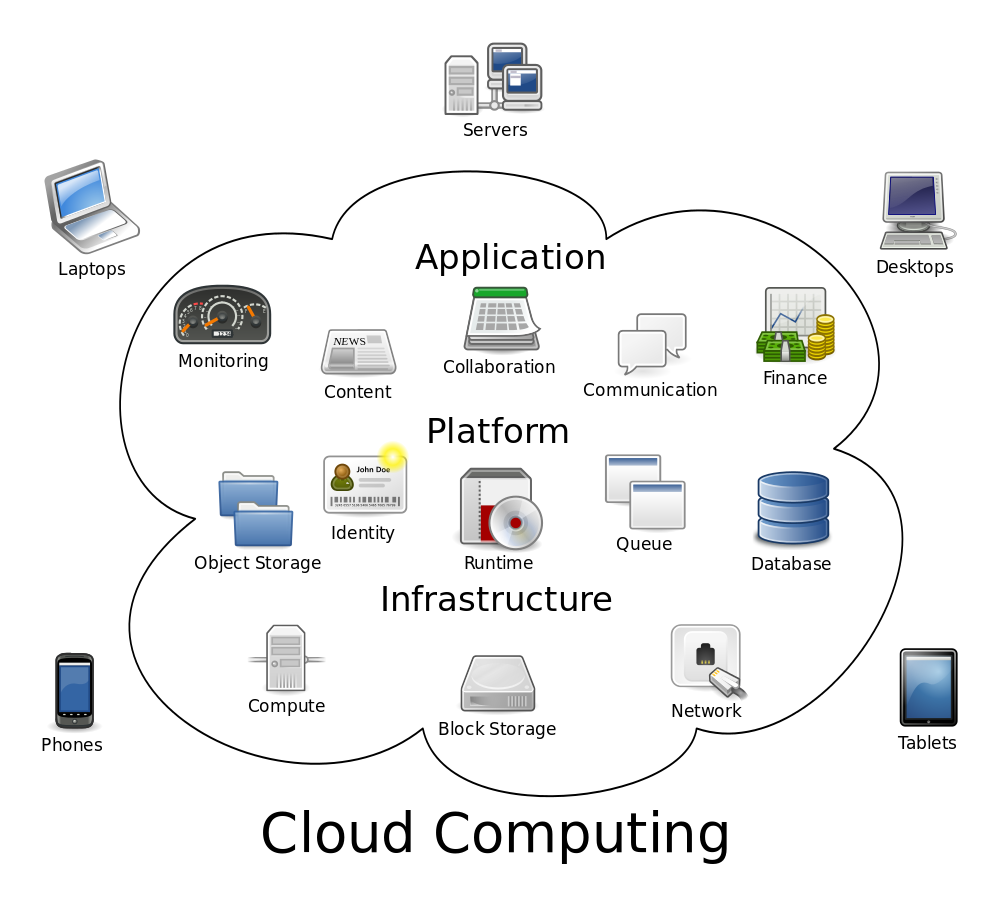
\includegraphics[width=\textwidth,height=0.8\textheight,keepaspectratio]{Cloud_computing.png}
  \end{figure}
\end{frame}

\begin{frame}
  \frametitle{Definition}
  \emph{NIST} provided a  description of the characteristics of a Cloud
  Computing infrastructure:
  \begin{itemize}
    \item On-demand Self-Service
    \item Broad Network Access
    \item Resource Pooling
    \item Rapid Elasticity
    \item Measured Services 
  \end{itemize}
\end{frame}

\begin{frame}
  \begin{figure}
    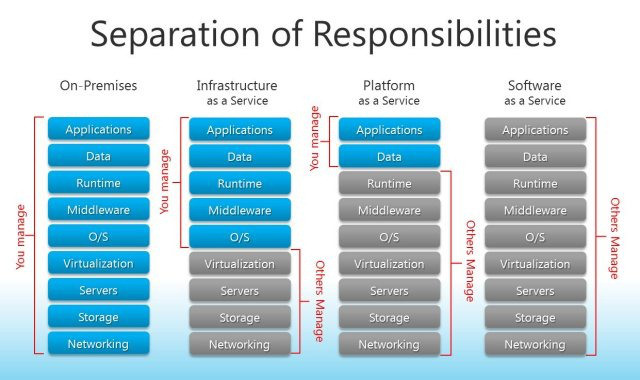
\includegraphics[width=\textwidth,height=0.8\textheight,keepaspectratio]{cloud_sep_of_resp.jpg}
  \end{figure}
\end{frame}

\subsection{Volunteer Cloud Computing}

\begin{frame}
  \frametitle{Volunteer Cloud Computing}
  \begin{itemize}
  \item Volunteer + Cloud = Volunteer Cloud Computing
  \end{itemize}
\end{frame}

\section{Related Work}
\begin{frame}
  \frametitle{Related Work}
  \begin{itemize}
  \item \textbf{Cloud@Home}[2009] and \textbf{Peer-2-Peer Cloud System}[2011]
  \item ... and a handful of conceptual reflections
  \end{itemize}
\end{frame}

\subsection{Cloud@Home}

\begin{frame}
 \frametitle{Cloud@Home}
     \begin{figure}[cathome]
      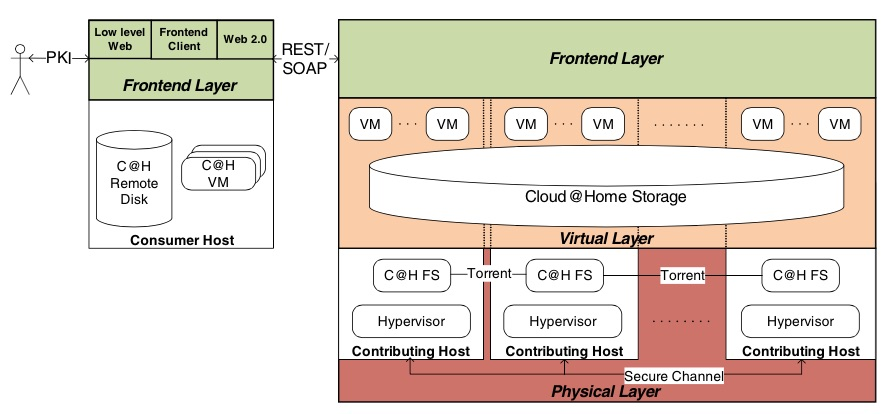
\includegraphics[width=\textwidth,height=0.8\textheight,keepaspectratio]{cathome_arch.jpg}
    \end{figure}
\end{frame}

\subsection{P2PCS}

\begin{frame}
  \frametitle{P2PCS}
  \begin{figure}
      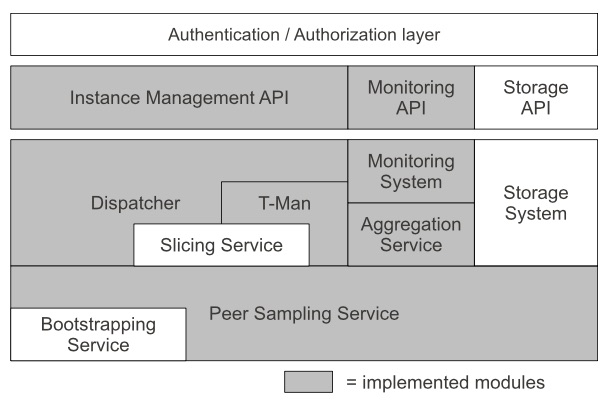
\includegraphics[width=\textwidth,height=0.8\textheight,keepaspectratio]{p2pcs_arch.jpg}
    \end{figure}
\end{frame}

\subsection{Analysis}

\begin{frame}
  \frametitle{Brief Analysis}
  \begin{itemize}
  \item \textbf{Scope}
  \item \textbf{Novelty} generally incurs under-specifications of the requirements!
  \end{itemize}
\end{frame}

\subsection{Requirements Definition}

\begin{frame}
  \frametitle{Requirements}
      \begin{figure}
      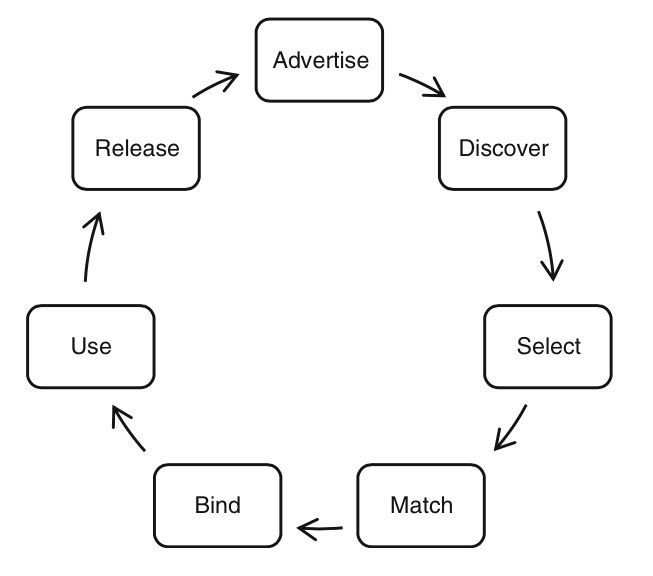
\includegraphics[width=\textwidth,height=0.8\textheight,keepaspectratio]{p2p-collab.jpg}
    \end{figure}
\end{frame}

\section{Infrastructure}
\subsection{Overview}
\begin{frame}
  \frametitle{Infrastructure}
  An Architecture for a fully de-centralized peer-to-peer volunteer
  cloud computing platform-as-a-service infrastructure.
  \tikzstyle{every node}=[draw=black,thick,anchor=west]
  \tikzstyle{selected}=[draw=red,fill=red!30]
  \tikzstyle{optional}=[dashed,fill=gray!50]
  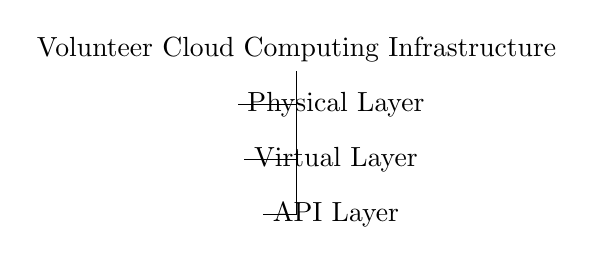
\begin{tikzpicture}[%
      grow via three points={one child at (0.5,-0.7) and
        two children at (0.5,-0.7) and (0.5,-1.4)},
      edge from parent path={(\tikzparentnode.south) |-
    (\tikzchildnode.west)}]
    \node {Volunteer Cloud Computing Infrastructure}
    child { node {Physical Layer}}
    child { node {Virtual Layer}}
    child { node {API Layer}};
  \end{tikzpicture}
\end{frame}  

\subsection{Physical Layer}
\begin{frame}
  \frametitle{Physical Layer}
  
  \tikzstyle{every node}=[draw=black,thick,anchor=west]
  \tikzstyle{selected}=[draw=red,fill=red!30]
  \tikzstyle{optional}=[dashed,fill=gray!50]
  \begin{tikzpicture}[%     
      grow via three points={one child at (0.5,-0.7) and
      two children at (0.5,-0.7) and (0.5,-1.4)},
    edge from parent path={(\tikzparentnode.south) |-
    (\tikzchildnode.west)}]
    \node {Physical Layer}
    child { node {Network Connectivity}
      child { node {Overlay Network}
        child { node [optional] {Structured Network}}
        child { node [optional] {Unstructured Network}}
    }};
  \end{tikzpicture}
\end{frame}

\subsection{Virtual Layer}
\begin{frame}
  \frametitle{Virtual Layer}
  \tikzstyle{every node}=[draw=black,thick,anchor=west]
  \tikzstyle{selected}=[draw=red,fill=red!30]
  \tikzstyle{optional}=[dashed,fill=gray!50]
    \begin{tikzpicture}[%                                                                                                                                                                                 
      grow via three points={one child at (0.5,-0.7) and
        two children at (0.5,-0.7) and (0.5,-1.4)},
      edge from parent path={(\tikzparentnode.south) |-
    (\tikzchildnode.west)}]
    \node {Virtual Layer}
    child { node {Virtualization}
      child {node [optional]{Light Virtualization}}
      child {node [optional]{Traditional Virtualization}}
    };
  \end{tikzpicture}
\end{frame}
\begin{frame}
  \begin{figure}                                                                                                                                                                                        
    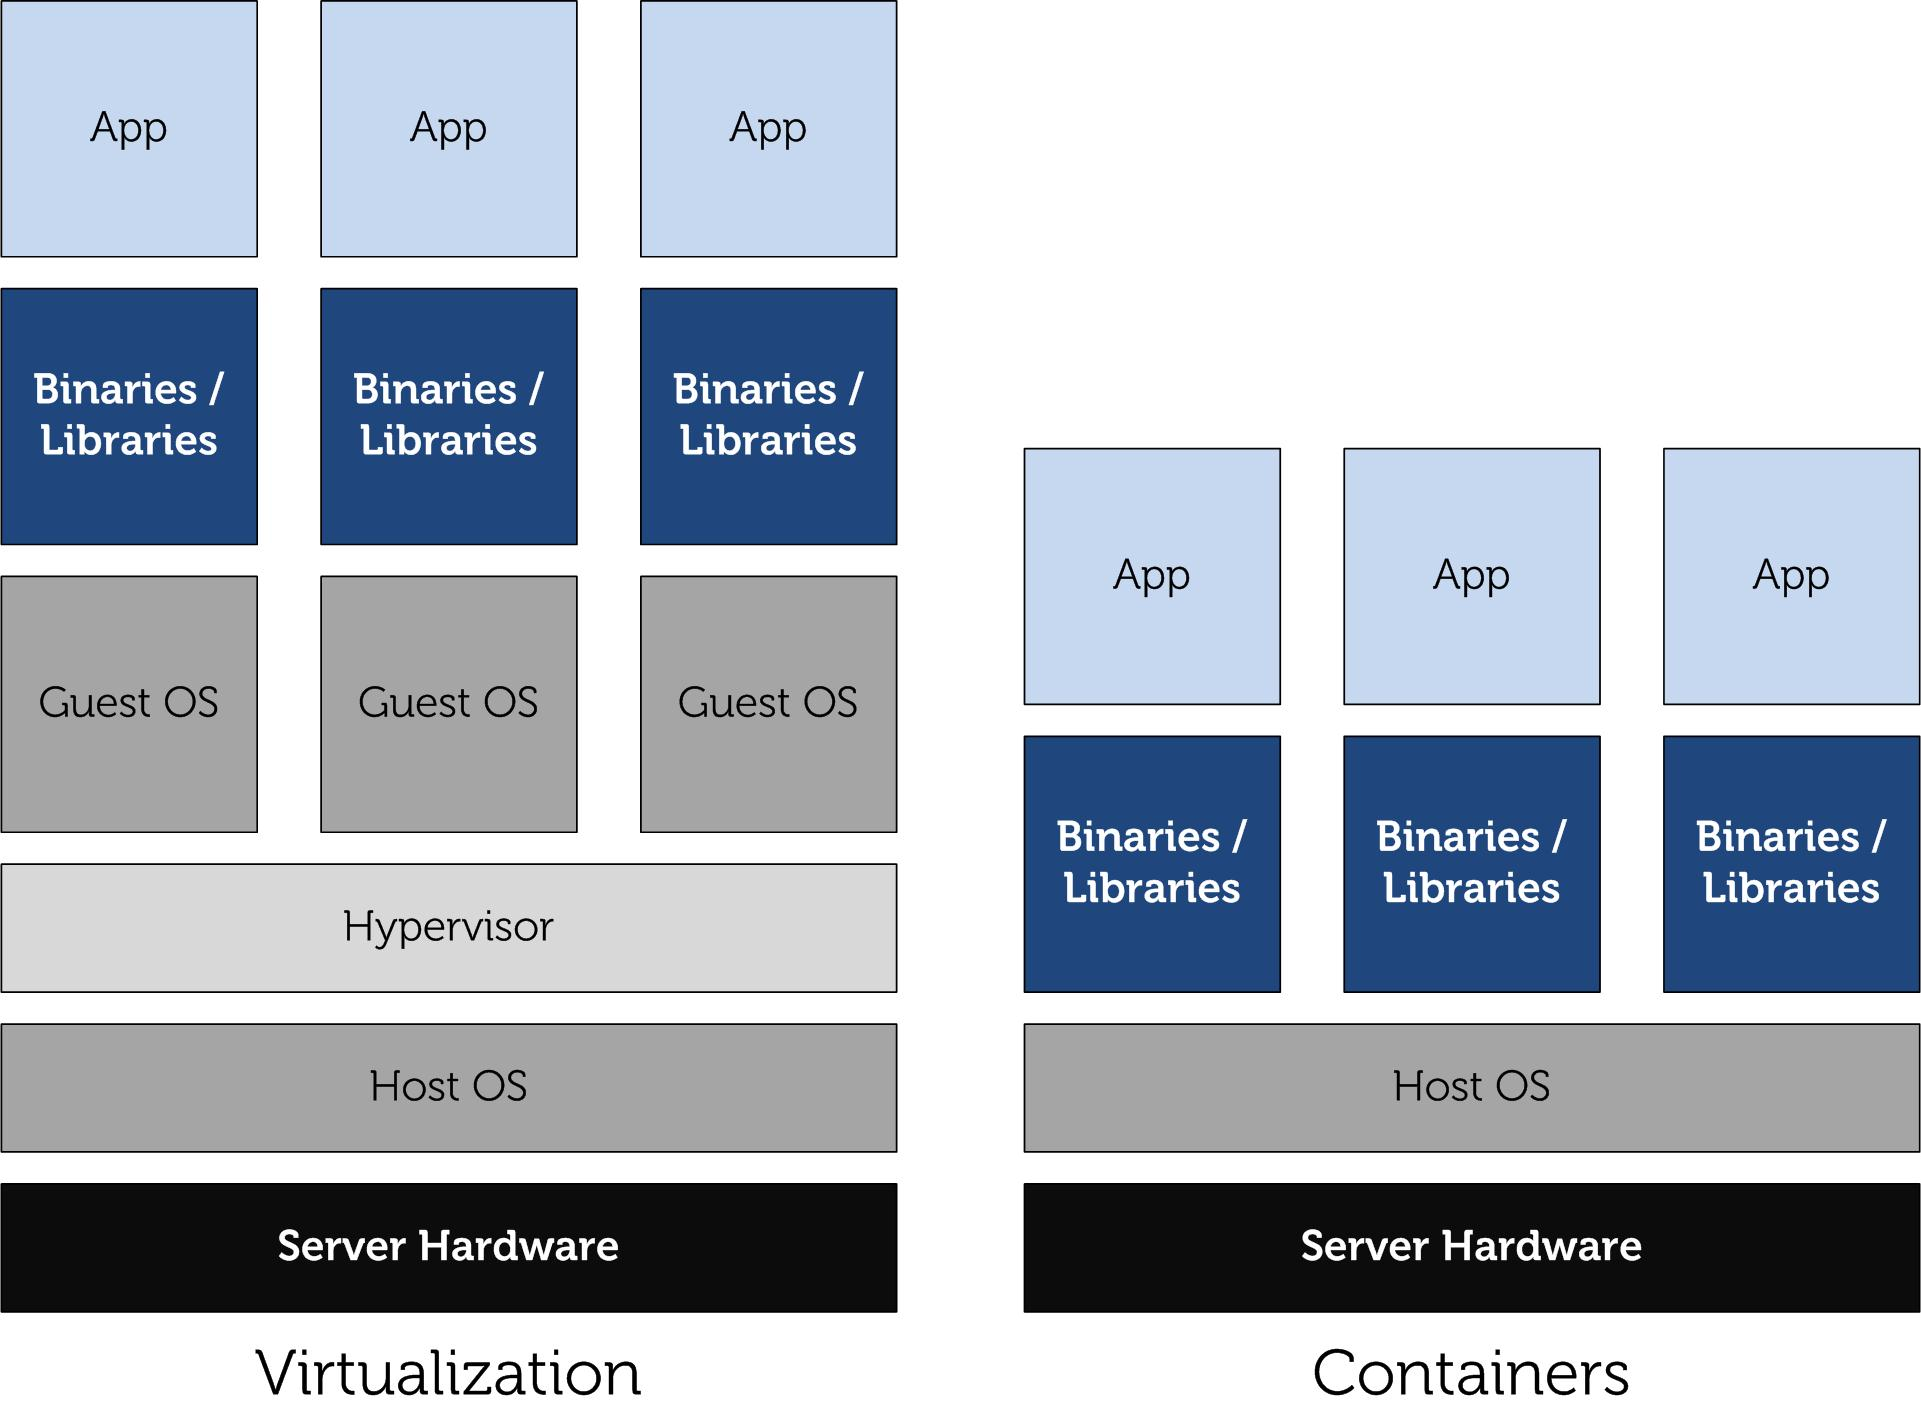
\includegraphics[width=\textwidth,height=0.8\textheight,keepaspectratio]{lxc-vm.jpg}                                                                                        
  \end{figure}
\end{frame}

\subsection{API Layer}
\begin{frame}
  \frametitle{API Layer}
  \tikzstyle{every node}=[draw=black,thick,anchor=west]
  \tikzstyle{selected}=[draw=red,fill=red!30]
  \tikzstyle{optional}=[dashed,fill=gray!50]    
  \begin{tikzpicture}[%                                                                                                                                                                                 
      grow via three points={one child at (0.5,-0.7) and
        two children at (0.5,-0.7) and (0.5,-1.4)},
      edge from parent path={(\tikzparentnode.south) |-
    (\tikzchildnode.west)}]
    \node {API Layer}
    child { node {Databases/Storages}}
    child { node {Front-End}}
    child { node [optional]{Load Balancing \& Scaling}}
    child { node {Security}}
    child { node [optional]{App. Deployment and Management}};
  \end{tikzpicture}
\end{frame}

\section{Open Problems}
\begin{frame}
  \begin{itemize}
    \item \textbf{Structured vs. Unstructured Networks} w.r.t. VCC
      (trade-off: Single-Attribute-Dominated Queries
      vs. Multi-Attribute-Dominated Queries).
    \item \textbf{Co-operative Web Hosting} how to host a web
      application using a peer-to-peer architecture.
  \end{itemize}
\end{frame}

\section{Contributions}
\begin{frame}
  \begin{itemize}
    \item \textbf{Using Light Virtualization rather than Traditional
      (VMs) Virtualization}
    \item \textbf{API Barebone specification}
    \item \textbf{Proof of concept, (work in progress...)}
    \item \textbf{Fully de-centralized approach to VCC}
  \end{itemize}
\end{frame}

\section{Future Work}
\begin{frame}
  \begin{itemize}
    \item Make the proof of concept closer to a production-ready
      prototype.
    \item Provide formal analysis of the F.T. and reliability of the
      system.
    \item Choose the most adequate solution (Physical Layer), rather
      than the most convenient. 
    \item Work towards a more concrete ontological representation of
      VCC.
  \end{itemize}
\end{frame}

\section{References}
\begin{frame}[allowframebreaks]
        \frametitle{References}
        \bibliographystyle{te}
        \tiny
        \bibliography{bibliography}
\end{frame}

\end{document}
